\section{Recovering Task-Relevant Structure through Compression}
\label{sec:recovery}

Section~\ref{sec:diagnostics} showed that compression acts unequally on the components of an update, and Section~\ref{sec:why-compression-helps} that removing or shrinking part of an update can improve on both the update and the frozen model. We test this by training adapters on corrupted data and compressing them. Our main corruption pairs each MetaMathQA question with the worked solution of another question, keeping its own final answer line. An adapter trained on these permuted rationales learns the answer format together with reasoning that does not match the question, and scores far below the frozen model.

\subsection{Compression repairs a damaged finetune}
Figure \ref{fig:families} shows the result of this process on three separate models. On Qwen2.5-7B, the permuted adapter drops GSM8K accuracy from 77.6\% to 23.7\%. Once lossily compressed to roughly 2.6MB and then uncompressed, this same adapter scores 82.9\%, not only beating the original corrupted adapter but also providing a notable gain over the base model's performance. This phenomenon reproduces with Mistral-7B-Instruct, leading to an even more impressive gain of 8.7\%, up from 15.4\% for the corrupted adapter. Llama-3.1-8B shows the same repair (19.8\% to 41.6\%), but its frozen base scores only 10\%, which is worse even than the corrupted adapter, as it struggles to stop generation to output an answer.


\begin{figure}[t]
\centering
    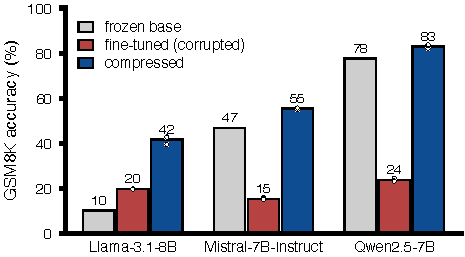
\includegraphics[width=0.62\linewidth]{figures/F5_families.pdf}
\caption{Compression recovers a damaged fine-tune independently in 3 separate models. For each, we plot GSM8K accuracy (1,319 problems) of the frozen base, of a corrupted adapter trained on permuted rationales, and of the same adapter after lossy compression to about 2.7 MB.}
\label{fig:families}
\end{figure}
% ANNEX: NF4, rank 16, permuted-rationale MetaMathQA (32k rows, 1 epoch), 1,319 GSM8K problems.
% Compressed = half the rank directions removed, the rest coded at 1 bit (2.63--2.74 MB).

There are two axes on which to compress: one can prune directions/ranks, code those directions more coarsely, or both, as shown in Figure~\ref{fig:rank-bits}. For a fixed budget $r \times b$ of up to 16, coding at 1 bit and keeping as many directions as the budget allows always scores best. The leading direction alone scores 81.4\% at 1 bit, above the base, but stays damaged at 16 bits (39.6\%); from a budget of 32 up, every combination is as damaged as the adapter itself. Further controls are in Appendix Table~\ref{tab:ladder}.



\begin{figure}[t]
\centering
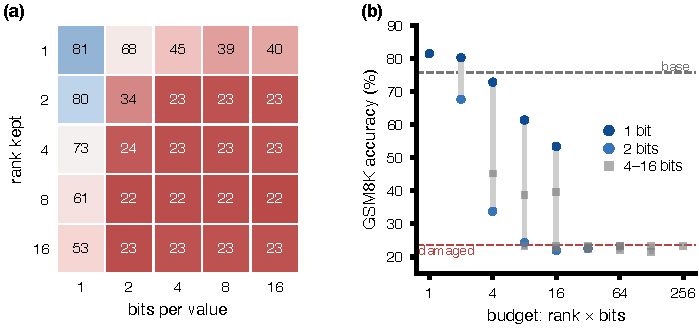
\includegraphics[width=0.85\linewidth]{figures/F4_rank_vs_bits.pdf}
\caption{Rank and precision are not interchangeable ways to spend bits. (a) GSM8K accuracy after cutting the corrupted rank-16 adapter to rank $r$ and coding it at $b$ bits per value; red is below the frozen base, blue above. (b) The same cells against the budget $r \times b$.}
\label{fig:rank-bits}
\end{figure}
% ANNEX: Qwen2.5-7B, NF4, permuted-rationale MetaMathQA, GSM8K 500, seed 11; frozen base 75.6. At budgets 4, 8 and 16 the
% cells spread by 39, 38 and 31 points and the 1-bit cell is always on top; from 32 up every cell sits at the damaged level.
% Rank 1 scores 81.4 at 1 bit and 39.6 at 16 bits. The 3-seed version of these controls is Table~\ref{tab:ladder} (appendix).

Coding at 1 bit acts mostly as shrinkage on the leading direction. By scaling the full-precision rank-1 update by a factore betweem 0.2 and 0.5, we get an accuracy of 80.8\%, level with the 1-bit code (80.2\%). Coding does have a positive effect on its own, with the coded update beating the rescaled one by 2.4 points at 1 bit and by 1.8 to 7.2 points at 2 to 8 bits, because coding also has an effect on the direction of the update. On the 72-probe panel of Section~\ref{sec:breadth}, this margin is small.

\begin{figure}[t]
\centering
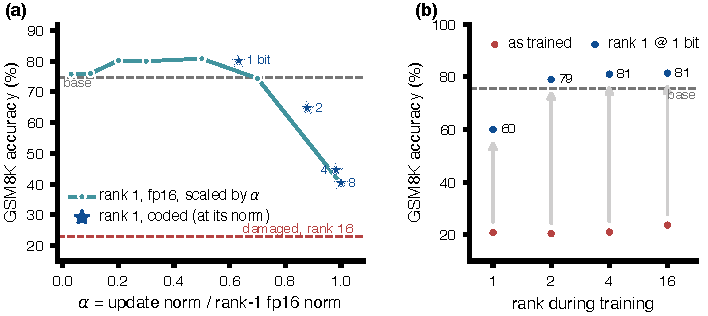
\includegraphics[width=0.9\linewidth]{figures/F6_shrinkage.pdf}
\caption{Coding the leading direction at 1 bit acts mostly as a shrinkage, and works only on an adapter trained wide. (a) The rank-1 update scaled by $\alpha$, against the coded updates at their own norm. (b) Adapters trained at rank 1, 2, 4 and 16 on the corrupted corpus all learn the damage (red); cut to rank 1 at 1 bit, the same 0.40 MB file, they reach 60.0, 79.0, 81.0 and 81.4 (blue). $\alpha/r=2$ throughout; Qwen2.5-7B, GSM8K 500, seed 11.}
\label{fig:shrinkage}
\end{figure}

For a compressed adapter to produce the repair effect over its corrupted baseline, the damage also needs to have been written into a wide enough adapter so it can be decomposed. Adapters trained directly at ranks 1 through 16 on the corrupted data consistently learned the damage, but once cut to rank 1 at 1 bit via a 0.40 MB file, adapters with larger initial ranks consistently showed largers gains than initially compact adapters (Figure~\ref{fig:shrinkage}b). This shows that compression is not equivalent to training a small adapter, as the useful components and damaging ones can only separate when the initial adapter has room to represent both.

\subsection{Corrupted adapters encode damage in their leading directions}

If a narrow corruption is written into the strongest directions of an update, the directions below them should carry the useful part. One can then expect three regimes: leading directions specific to the training set, such as a precise output structure; a middle regime of task-level behavior, such as the form of a chain of thought; and a tail that adds little. Keeping only the middle regime should recover the task without any coding. We verify this in Figure~\ref{fig:r6r7}, where we score every contiguous window $[i, j)$ of the 16 singular directions of a corrupted adapter at full precision on 128 reserved MetaMathQA problems. We then compute, on average, the average impact on accuracy of a given singular direction. Experimentally, we do see the presence of three separate regimes, with initial directions being harmful, "centered" directions being most helpful, and later directions being neither helpful nor unhelpful.
It should be noted the larger the model, the smaller the improvement our corrupted adapter tended to provide over the baseline; and the wider the band of singular directions encoding harmful changes tended be. Our adapters being limited to rank 16, in particular, ended up cropping out the later part of the second band on Qwen2.5-32B. This is likely due to the greater intrinsic dimensionality of representations of larger models; further tests on more difficult tasks and adapter of higher rank would be a natural continuation of this work.


\begin{figure}[h]
\centering
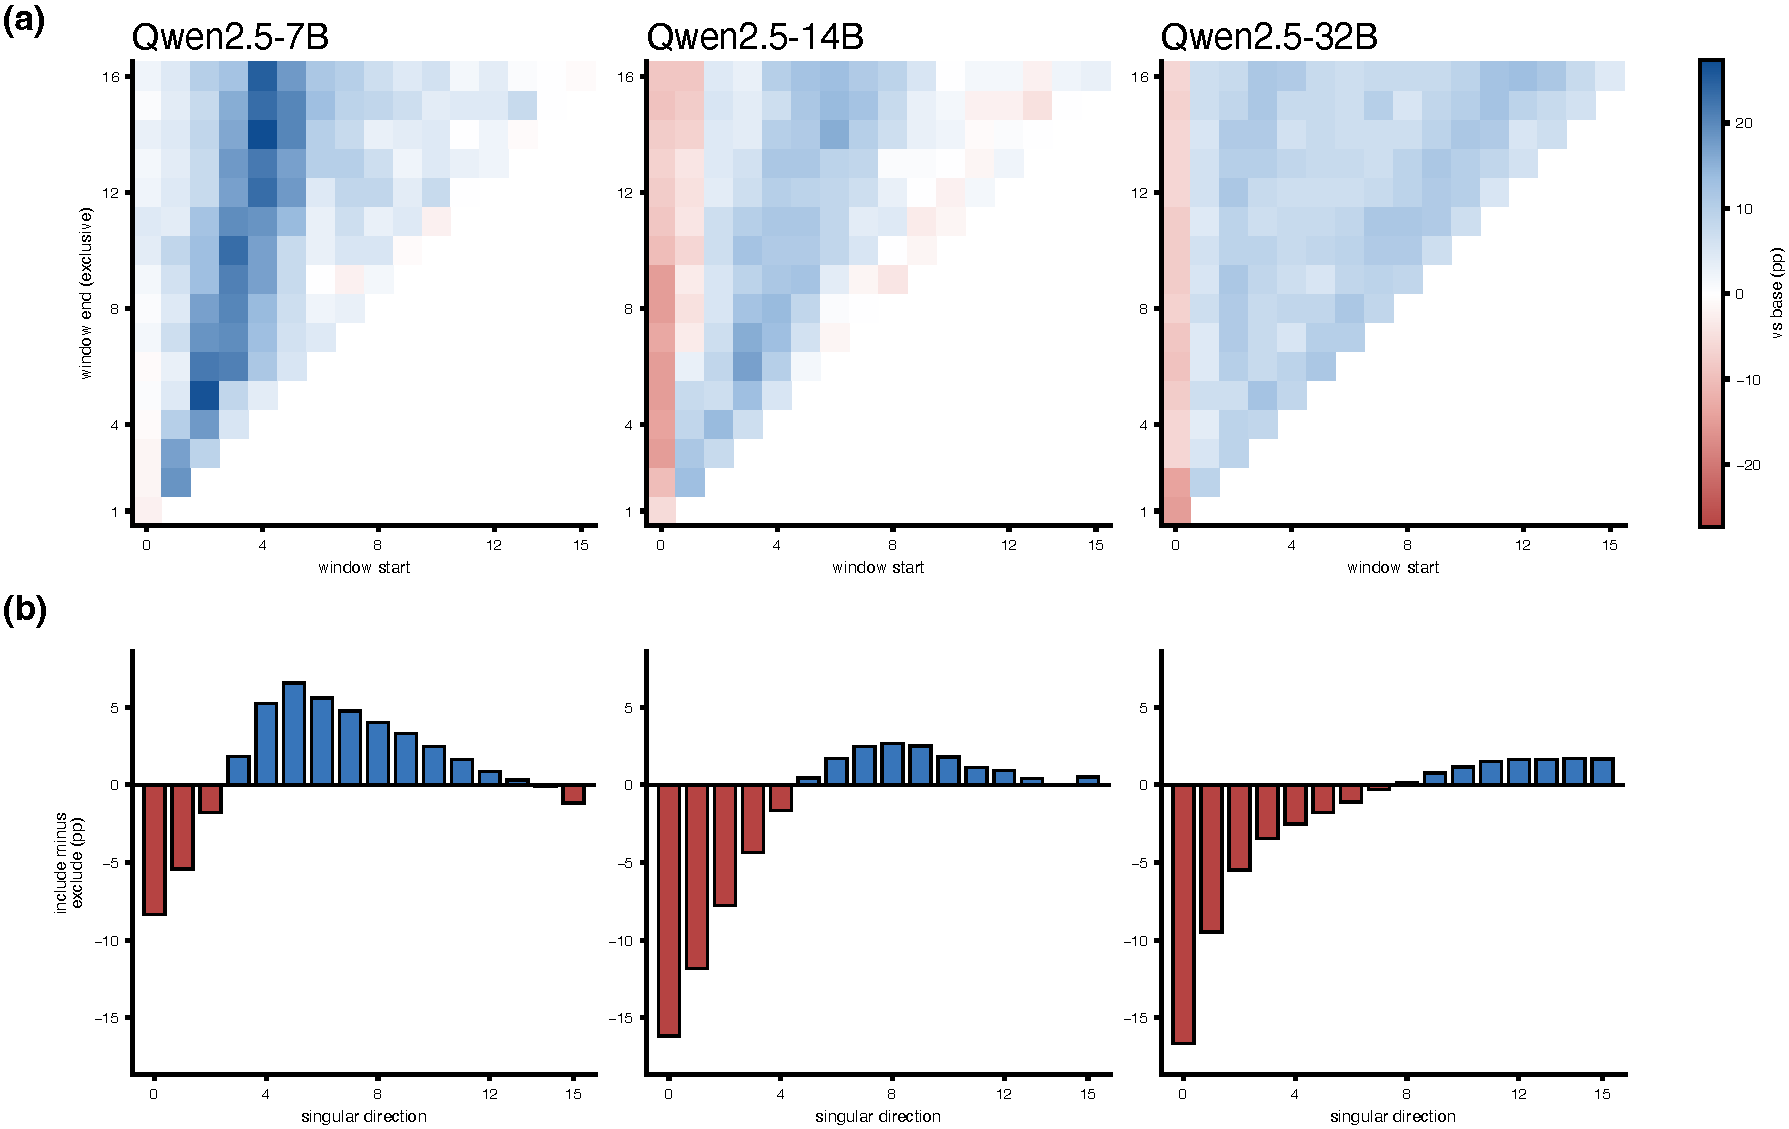
\includegraphics[width=0.85\linewidth]{figures/R6R7_collage.pdf}
\caption{SVD pass-band across scale, highlighting the existence of different regimes of directions. (a) Accuracy minus base for every window $[i,j)$ of singular directions kept at full precision. (b) For each direction, mean accuracy of the windows that contain it minus that of the windows that do not.}
\label{fig:r6r7}
\end{figure}

\subsection{Scaling}

In our experiments, the repair effects of compression hold across scale, model family and type of task. It is naturally harder for compressed adapters to establish a significant gain over baseline as the baseline gets closer and closer to saturating a dataset. 

\begin{table}[t]
\caption{Damage and repair across scale (Qwen2.5). Up to 7B: GSM8K accuracy (\%), permuted rationales. 14B, 32B: XBRL tagging exact match, each response dealt to another filing; mismatched tags still teach the tag vocabulary, so there the corrupted adapter beats the weak base.}

\label{tab:scale}
\centering
\small
\begin{tabular}{lrrrrr}
\toprule
size & base & damaged & clean & rank 1 @ 1 bit & overshoot \\
\midrule
0.5B & 23.0 & 9.4 & 45.2 & 25.0 & +2.0 \\
1.5B & 51.6 & 13.6 & 67.6 & 59.0 & +7.4 \\
3B & 60.4 & 17.4 & 74.0 & 71.0 & \textbf{+10.6} \\
7B & 75.6 & 22.8 & 81.0 & 80.8 & +5.2 \\
\midrule
14B, XBRL tagging & 24.6 & 53.0 & -- & 73.8 & +49.2 \\
32B, XBRL tagging & 32.4 & 51.8 & -- & 74.4 & +42.0 \\
\bottomrule
\end{tabular}
\end{table}
% ANNEX: NF4, rank 16, one seed. GSM8K rows: permuted-rationale MetaMathQA, 500 test questions; the 7B clean value comes
% from a separate GSM8K run whose base scores 75.6. GSM8K at 14B / 32B (removed from the table): base 84.0 / 91.0, damaged
% 37.4 / 39.6, clean 83.6 / 85.0, rank 1 @ 1 bit 81.8 / 86.8. XBRL rows: headroom grid (results/tasks/headroom_grid.csv),
% 500 test rows; directions 4-15 score 66.4 / 74.6. Pointer chasing 32B: base 80.0, damaged 1.2, rank 1 @ 1 bit 12.2.

\subsection{Generalization}
\label{sec:breadth}

A fine-tune also changes performance on tasks it was not trained on. We compare the clean and compressed corrupted adapters on 72 probes at increasing distance from their training task. Section~\ref{sec:why-compression-helps} predicts that a compressed update moves the model less off-task. Figure~\ref{fig:breadth} confirms it: the two adapters are matched on GSM8K but differ sharply away from it. On tasks related to common sense, code or humanities, the compressed adapter matches the performance of the base level, whereas the clean adapter already drops in performance. On different, harder math  such as MATH-500, AQuA and MMLU mathematics, the clean adapter keeps 44\% of the base accuracy and the compressed one 97\%.


\begin{figure}[t]
\centering
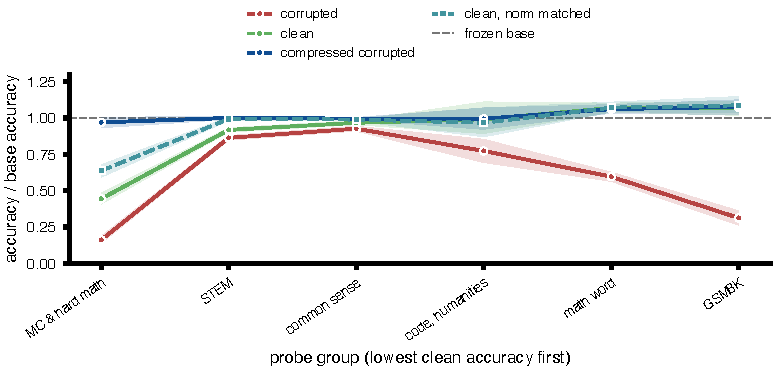
\includegraphics[width=0.65\linewidth]{figures/F9_breadth.pdf}
\caption{The compressed corrupted adapter stays at the base away from its task; the clean adapter does not, even when norm-matched to the compressed adapter. Accuracy on 72 probes divided by the frozen Qwen2.5-7B base accuracy, grouped by distance from GSM8K.}
\label{fig:breadth}
\end{figure}